%%
%% This is file `sample-authordraft.tex',
%% generated with the docstrip utility.
%%
%% The original source files were:
%%
%% samples.dtx  (with options: `authordraft')
%% 
%% IMPORTANT NOTICE:
%% 
%% For the copyright see the source file.
%% 
%% Any modified versions of this file must be renamed
%% with new filenames distinct from sample-authordraft.tex.
%% 
%% For distribution of the original source see the terms
%% for copying and modification in the file samples.dtx.
%% 
%% This generated file may be distributed as long as the
%% original source files, as listed above, are part of the
%% same distribution. (The sources need not necessarily be
%% in the same archive or directory.)
%%
%% Commands for TeXCount
%TC:macro \cite [option:text,text]
%TC:macro \citep [option:text,text]
%TC:macro \citet [option:text,text]
%TC:envir table 0 1
%TC:envir table* 0 1
%TC:envir tabular [ignore] word
%TC:envir displaymath 0 word
%TC:envir math 0 word
%TC:envir comment 0 0
%%
%%
%% The first command in your LaTeX source must be the \documentclass command.
\documentclass[sigconf, anonymous, review]{acmart}
\acmSubmissionID{967}
\usepackage[mathscr]{euscript}
%% NOTE that a single column version may required for 
%% submission and peer review. This can be done by changing
%% the \doucmentclass[...]{acmart} in this template to 
%% \documentclass[manuscript,screen]{acmart}
%%
\usepackage{algpseudocode}
\usepackage{algorithm,colortbl,xcolor}
\definecolor{Gray}{gray}{0.85}

\AtBeginDocument{%
  \providecommand\BibTeX{{%
    \normalfont B\kern-0.5em{\scshape i\kern-0.25em b}\kern-0.8em\TeX}}}

\begin{document}

%%
%% The "title" command has an optional parameter,
%% allowing the author to define a "short title" to be used in page headers.
\title{Supplemental Material for `Group Testing for Accurate and Efficient Nearest Neighbor Search: An Adaptive Binary Splitting Approach'}

%%
%% The "author" command and its associated commands are used to define
%% the authors and their affiliations.
%% Of note is the shared affiliation of the first two authors, and the
%% "authornote" and "authornotemark" commands
%% used to denote shared contribution to the research.

%%
%% By default, the full list of authors will be used in the page
%% headers. Often, this list is too long, and will overlap
%% other information printed in the page headers. This command allows
%% the author to define a more concise list
%% of authors' names for this purpose.
\maketitle

\section{Contents}
This supplemental material contains a figure showing the negative logarithm of the normalized histograms of dot products between feature vectors of query images and those of all gallery images from each of the five datasets we experimented with in the main paper. These are shown in Fig.~\ref{fig:histograms_dotproducts}. Compare with Fig. 2 of the main paper where normalized histograms are shown. We also show an additional result with the \textsc{Flinng} method from \cite{Engels2021} in Table~\ref{tab:KNN_flinng}. Here, the recall values for $K = 100$ nearest neighbors from
$K'=10^5$ retrieved neighbors are shown. 

\begin{figure*}
    \centering
    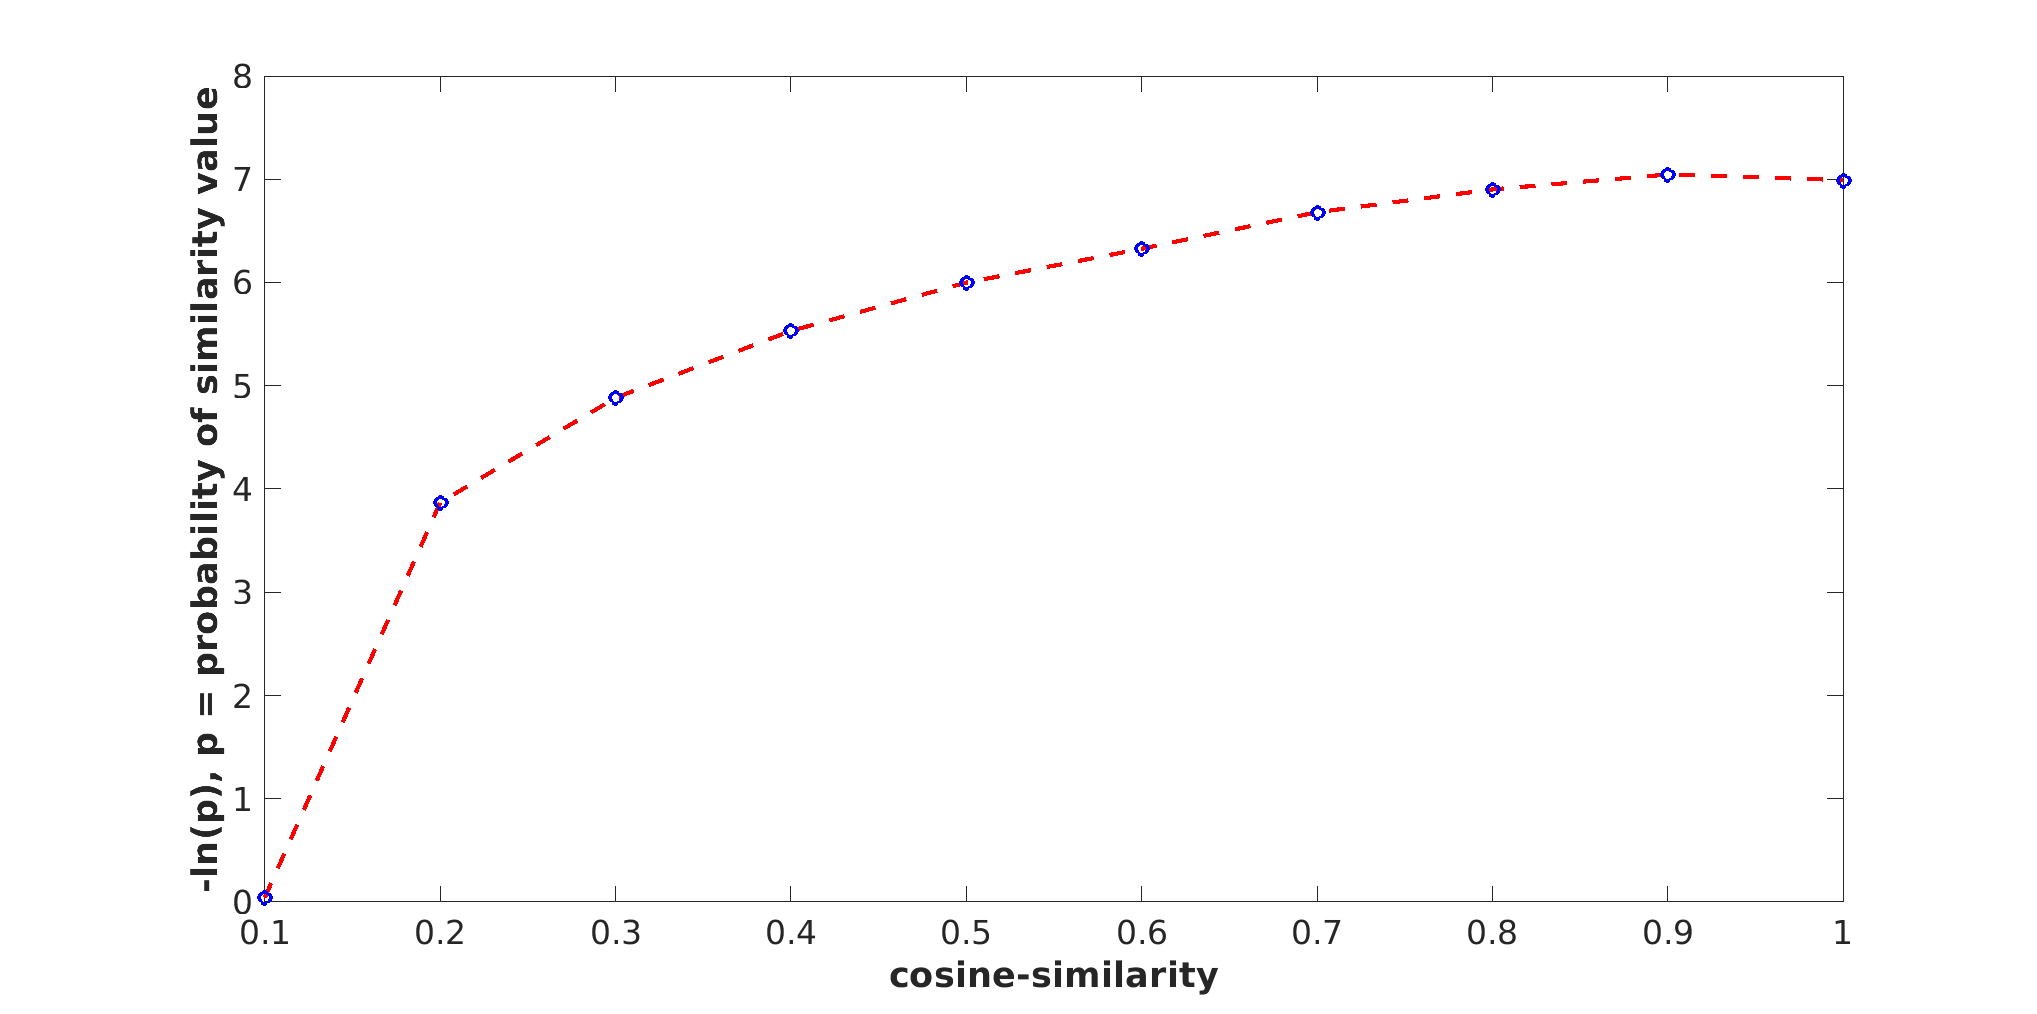
\includegraphics[scale=0.22]{figs/dotProducts_MIRFLICKR_1m.png}
    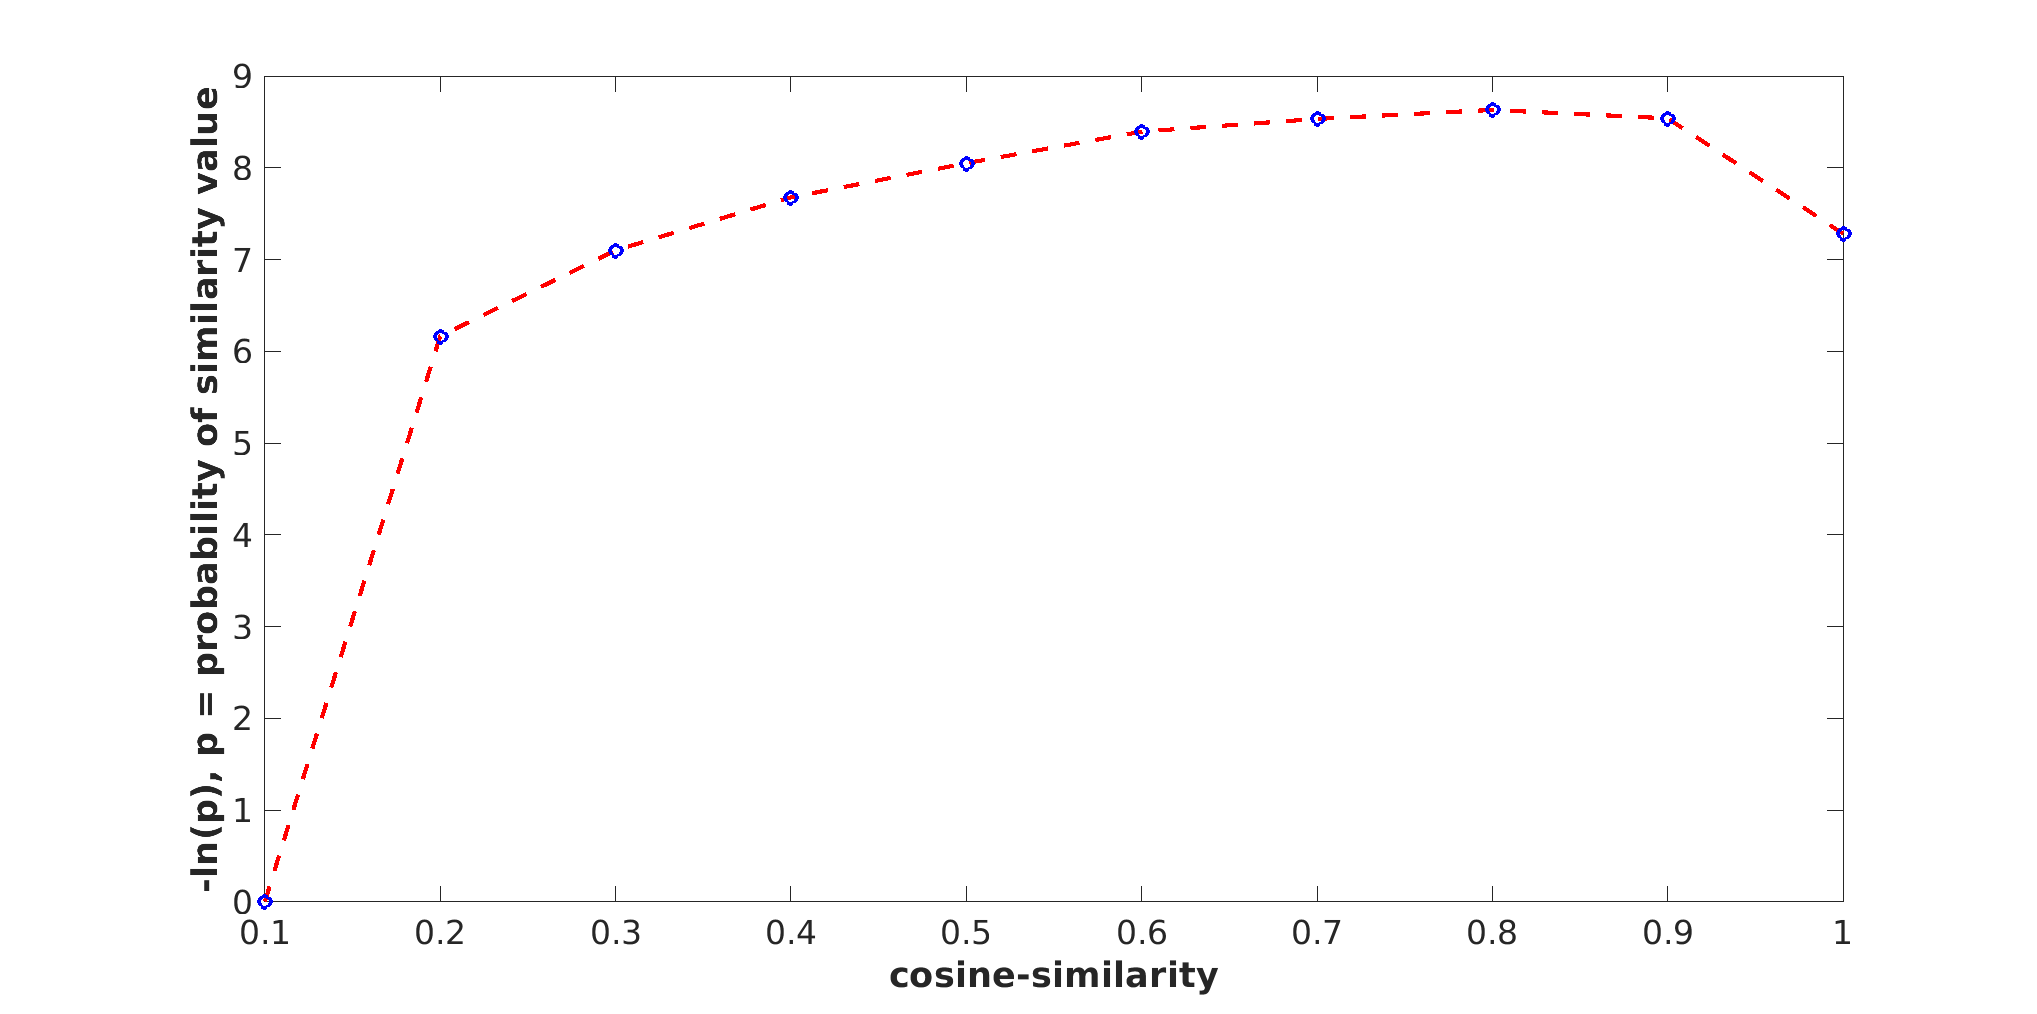
\includegraphics[scale=0.22]{figs/dotProducts_imageNet.png}
    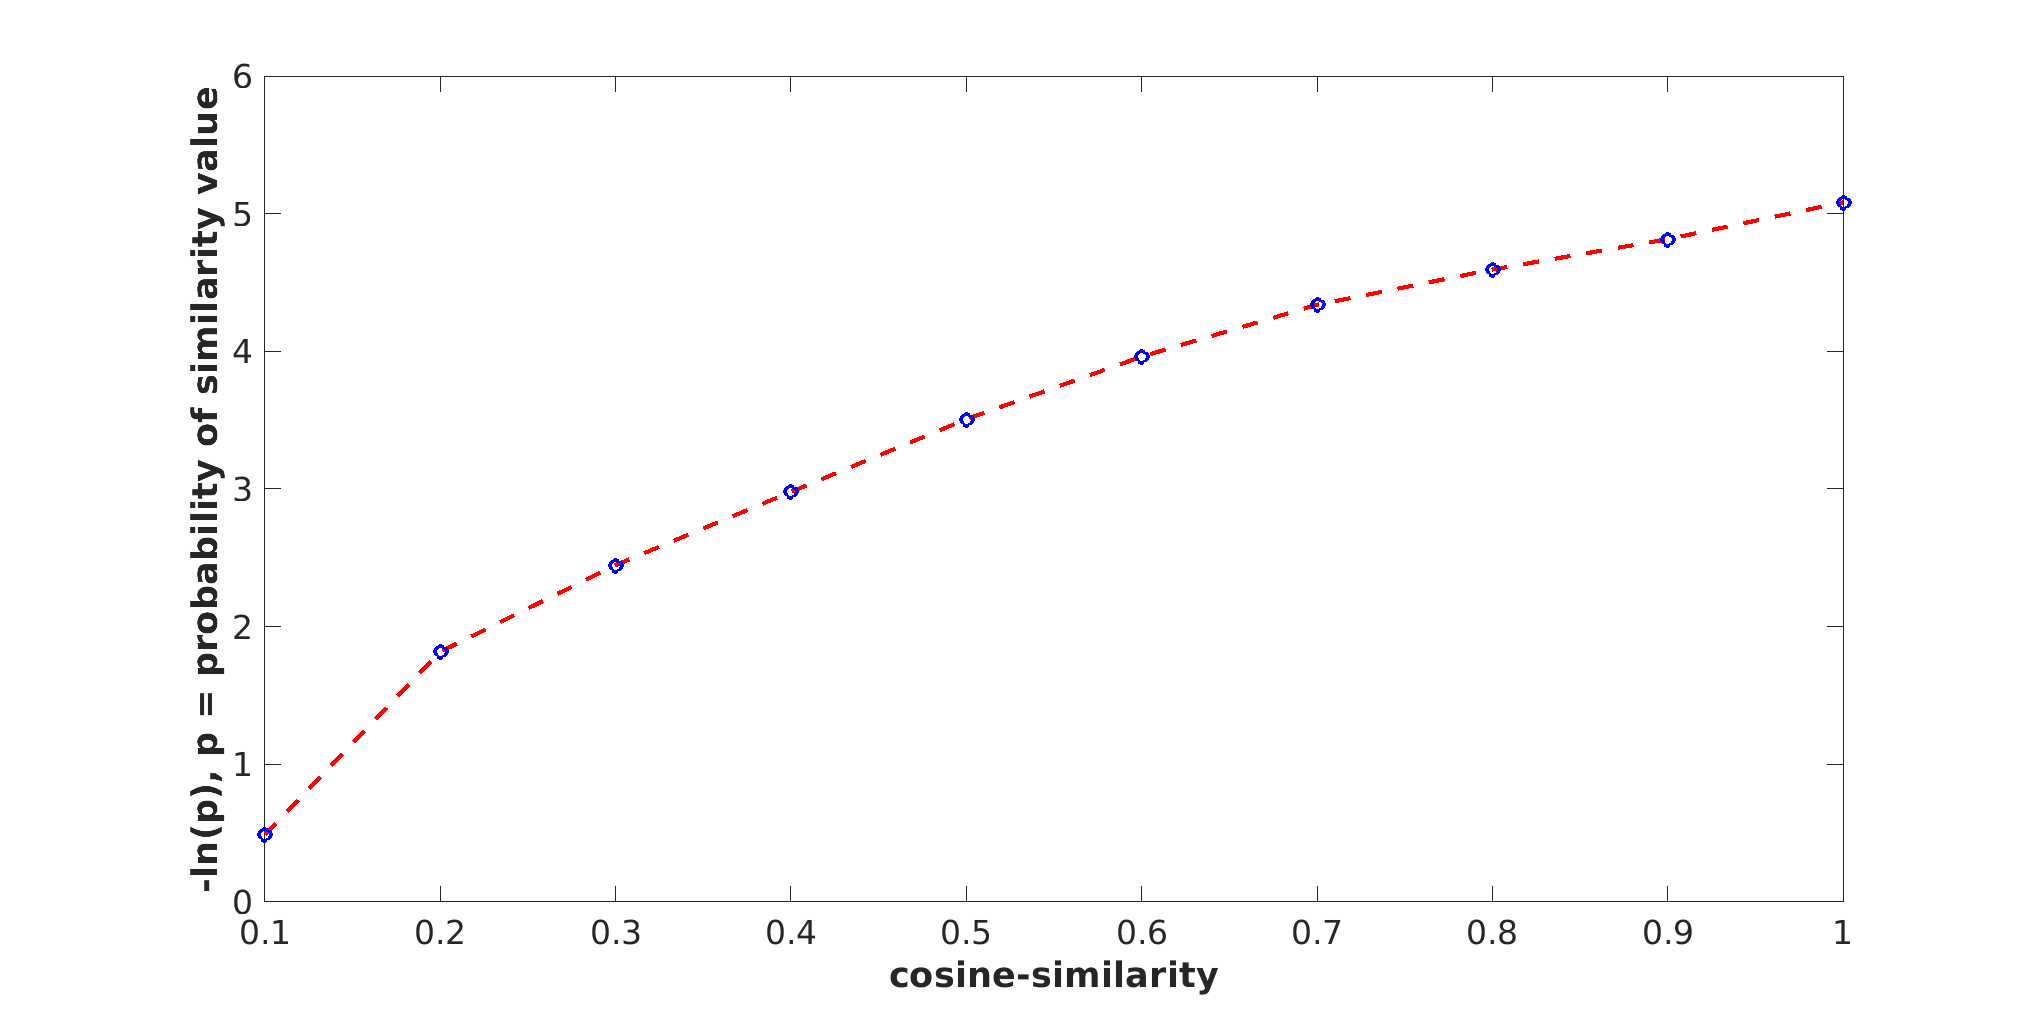
\includegraphics[scale=0.22]{figs/dotProducts_imdb_wiki.png}
    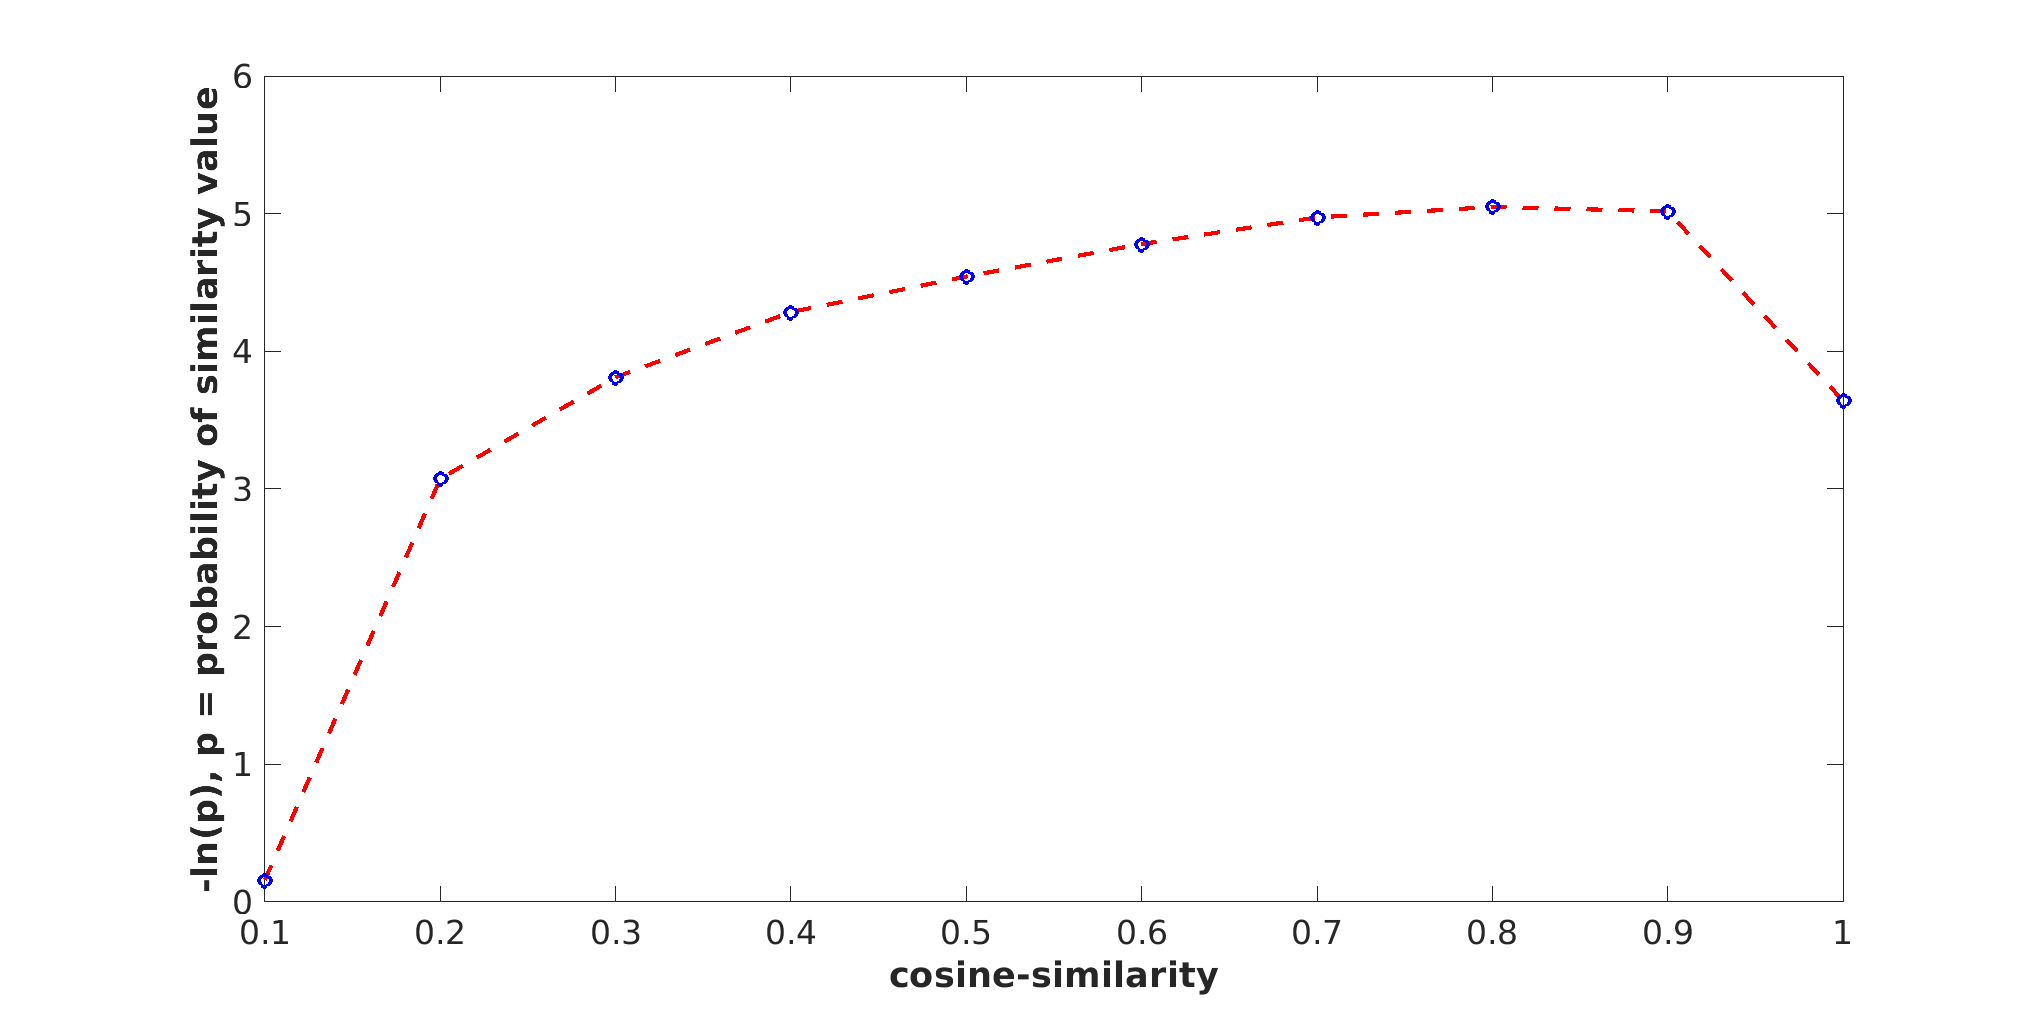
\includegraphics[scale=0.22]{figs/dotProducts_glami_1m.png}
    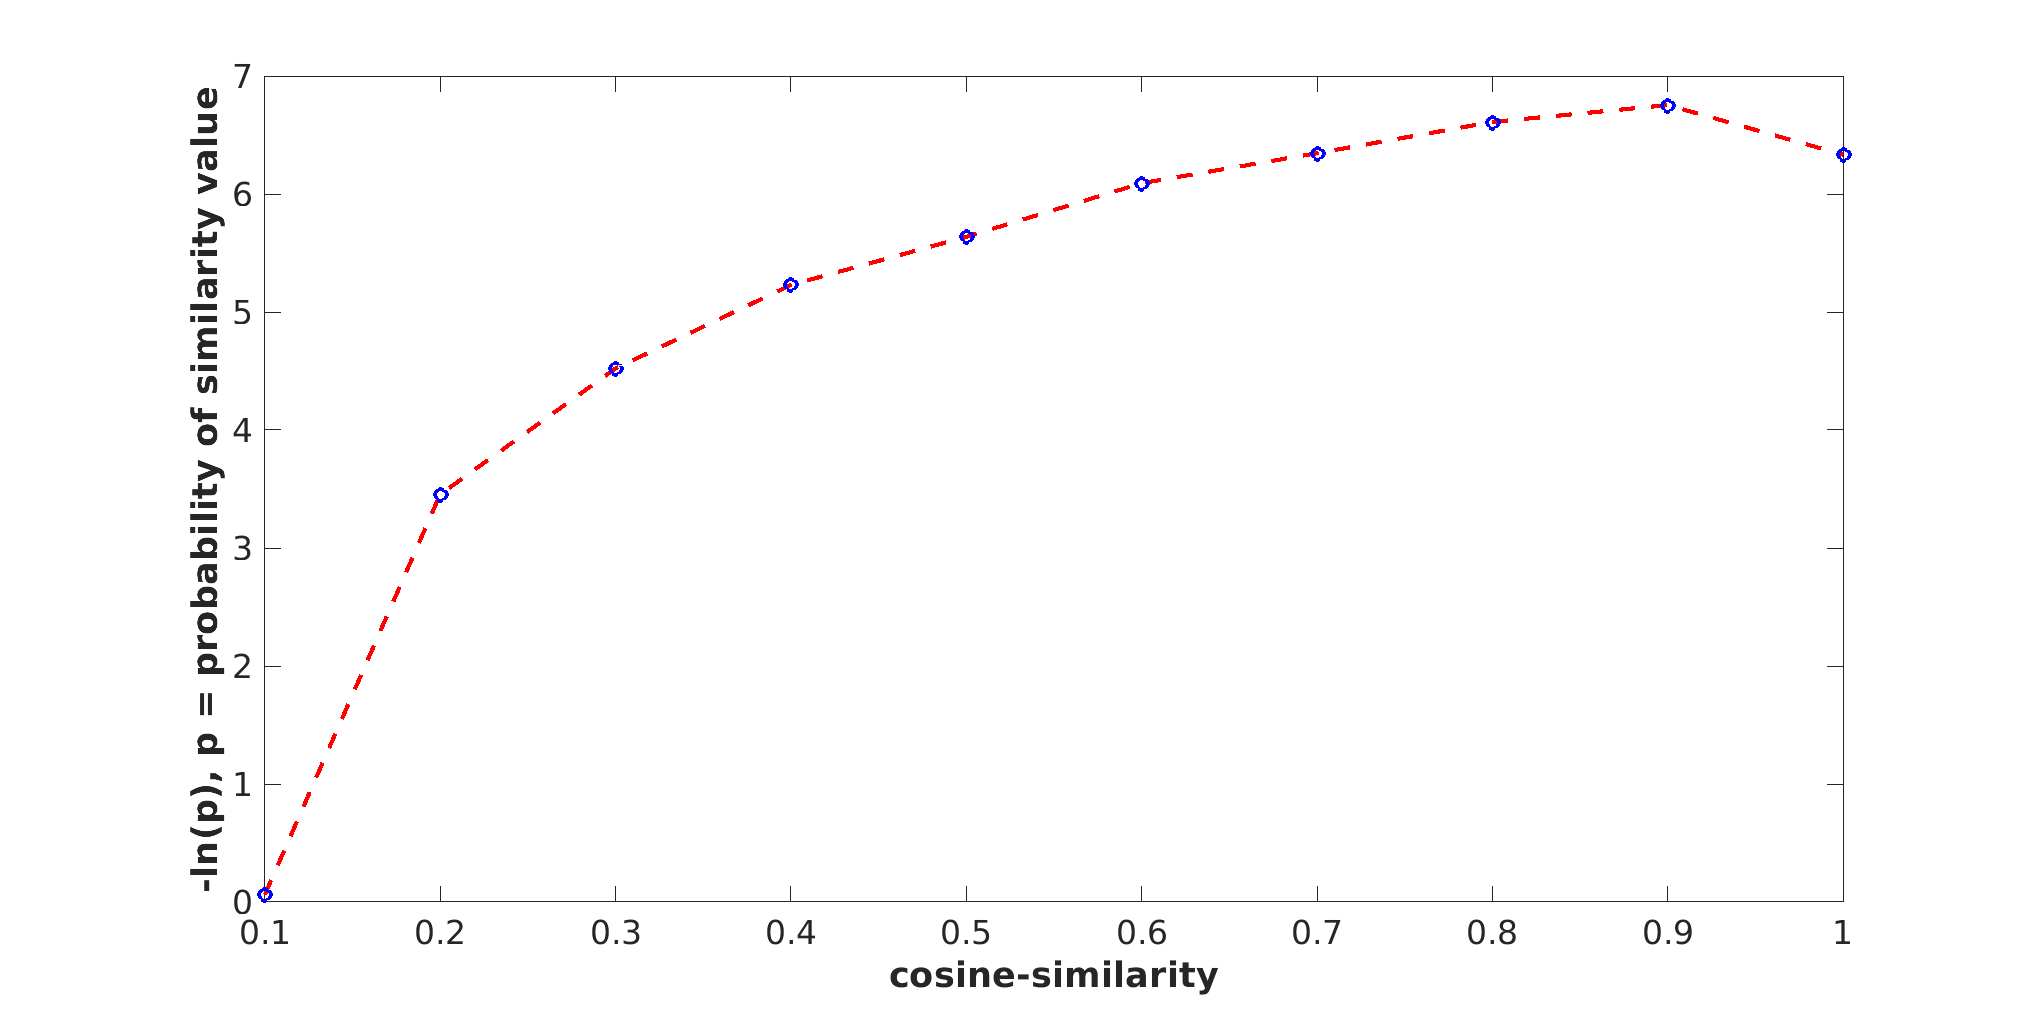
\includegraphics[scale=0.22]{figs/dotProducts_instaC_1m.png}
    \caption{Negative logarithm of normalized histograms of dot products between feature vectors of query images (10K in number) and those of all gallery images of MIRFLICKR, ImageNet, IMDB-Wiki, GLAMI and InstaCities (left to right, top to bottom).}
    \label{fig:histograms_dotproducts}
\end{figure*}

\begin{table*}
    \centering
    \begin{tabular}{|c|c|}
    \hline \rowcolor{Gray}
         Dataset & Recall for $K=100$ neighbors from $K'=10^5$ retrieved neighbors \\\hline
         \textsf{MIRFLICKR} & 0.866\\\hline
         \textsf{ImageNet} & 0.908\\\hline
         \textsf{IMDB-Wiki} & 0.9586\\\hline
         \textsf{GLAMI} & 0.9563\\\hline
         \textsf{InstaCities} & 0.875\\\hline
    \end{tabular}
    \caption{Recall values for different datasets with the \textsc{Flinng} \cite{Engels2021} for finding top $K=100$ nearest neighbors out of $K'=10^5$ retrieved neighbors.}
    \label{tab:KNN_flinng}
\end{table*}


\bibliographystyle{ACM-Reference-Format}
\bibliography{sample-base}

\end{document}
\endinput
%%
%% End of file `sample-authordraft.tex'.
